
\chapter{Security Administrator}
\label{SA}

\section{Security Operations}
\label{SA:SO}

Operazioni relative alla sicurezza:
\begin{itemize}
\item Gestione delle identità e controllo degli accessi: per esempio badge 
all'ingresso ecc. Ma non solo! Anche controlli di tipo informatico devono
essere aggiornati dopo ad esempio il licenziamento di un impiegato, al quale
dev'essere negato l'accesso ai dati aziendali alla fine del suo ultimo giorno
lavorativo;
\item \textit{Patching} del sistema e gestione delle configurazioni: il
patching è l'anno zero della sicurezza;
\item Controlli dei cambiamenti e gestione dei rilasci: Il controllo dei 
cambiamenti ogni cambiamento deve essere documentato e i test sono stati 
eseguiti allora può essere introdotto.
I rilasci software devono essere prima di tutto testati e documentati, e poi
devono essere autorizzati dall'apposito responsabile. Questo procedimento
garantisce che il software introdotto nel sistema non causi anomalie;
\item Metriche per la sicurezza e reporting: Ogni società sa dove bisogna 
andare. Una tipica metrica di sicurezza in caso di \emph{awareness} interna,
consiste nel mandare false email di spam ai dipendenti per vedere se
hanno recepito le lezioni sulla sicurezza;
\item Mantenimento dei controlli tecnologici: i controlli vanno mantenuti. 
Il controllo di sicurezza è un qualcosa che da un risparmio in termini di costi 
se applicata in maniera efficace. Vendere la sicurezza è difficile, e un buon 
manager è in grado di venderla;

\item Risposta all'incidente, investigazione e conseguente risoluzione
Il problema non è come si viene attaccati ma quando si è attaccati: bisogna 
avere un buon grado di comunicazione e trovare la causa dell'incidente. Anche 
avere una buona soluzione, per prevenire che l'incidente si verifichi di nuovo.
\textit{Investigation} è la fase successiva all'attacco e serve per capire 
perché e come è successo quello che è successo.

\end{itemize}


\subsection{IS Auditor e IT Governance}

Esistono cinque indicatori per capire se l'azienda ha fatto un buon lavoro nel 
veicolare i propri obiettivi ai lavoratori. È importante che i dipendenti 
sappiano dare risposte a cosa è allineata la compagnia, qual è la sua missione, 
visione, valori, obiettivi e strategie. Quando un dipendente non lo sa o 
risponde ``solo per i soldi'' è un segnale negativo.

\paragraph*{IT} L'IT serve per potare avanti obiettivi strategici di business, 
ed è importante sapere se l'IT è in grado di raggiungere le \textit{performance}
e gli obiettivi stabiliti. Inoltre sono presenti requisiti a cui essi devono 
sottostare, come per esempio quelli legali o quelli legati alla qualità.

\paragraph*{Efficacia ed efficienza} L'efficienza è l'uso ottimale delle 
risorse, l'efficacia è il raggiungimento degli obiettivi e dei requisiti 
prefissati.


\subsection{Esercizi}

La parte di esercizi è disponibili in \ref{esSA:SO}

\part{Controlli di Sicurezza e Sicurezza del Software}

Questo modulo si concentra sui controlli di sicurezza del software. Per fare ciò 
dovremo vedere il ciclo di vita del software, con un occhio alla sicurezza.
Partiremo dall'analisi dei requisiti, per andare all'analisi del rischio e per 
finire con lo sviluppo del software.
Anche l'ambiente produttivo richiede attenzione: è importante il mantenimento da 
parte di vista della sicurezza per non introdurre bug nel software.

\begin{figure}[h!]
        \begin{center}
                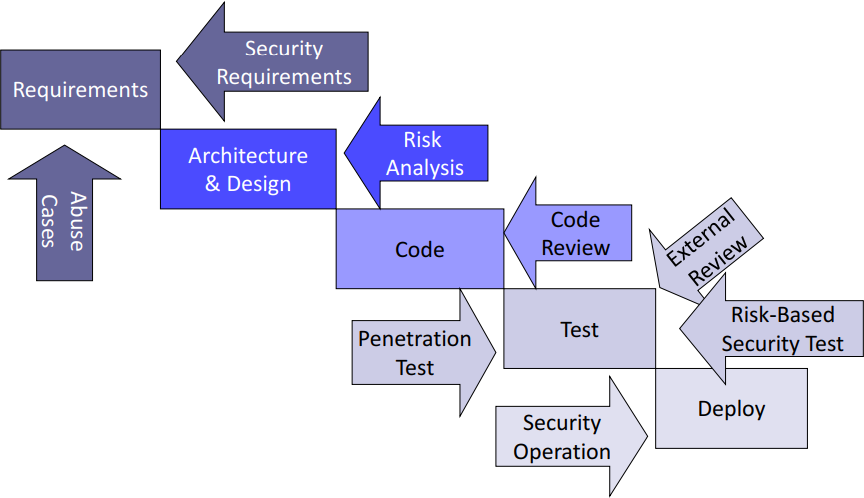
\includegraphics[width=\textwidth]{security_software_development}
        \end{center}
        \caption[La sicurezza nello sviluppo del software]{
         La sicurezza nello sviluppo del software. Nella figura
         \begin{enumerate*}[label=\alph*)]
		 \item ``Abuse cases'' (invece di use cases) si riferiscono ai
		 tipici casi in cui il sistema può essere flesso in chiara 
		 violazione delle policy di sicurezza;
		 \item La Code review consiste anche nell'analisi statica;
		 \item Il Test sul software è inteso come penetration test, stress test, ecc.
		 \end{enumerate*}
		}
        \label{fig:security:software:development}
\end{figure}

Prima di procedere con lo studio dei vari controlli nei capitoli
\ref{cs:ac} e \ref{cs:aa}, analizzeremo nell'ambito del capitolo 
\ref{Controlli} come si è evoluto il software e i conseguenti attacchi, 
a partire da attacchi classici come il \textit{buffer overflow}, 
per arrivare a sfruttare errori nella codifica dei caratteri negli URL
degli indirizzi web.

\chapter{Controlli}
\label{Controlli}

\section{Controlli su input}

Ci sono diversi tipi di attacchi che sfruttano gli input, e questi sono: 
\textbf{dati falsi}, \textbf{buffer overflow}\footnote{Si sfrutta l'allocazione 
di memoria nei programmi per eseguire codice arbitrario. Molto difficile da 
applicare ma molto efficace una volta riuscito l'attacco. Da spesso la 
possibilità all'attaccante di ottenere il controllo della macchina. Vedere il 
paper: \textit{Smashing The Stack For Fun And Profit.}}.

Per risolvere tutti questi problemi è necessario \textbf{validare l'input}, 
meglio se tramite le \textit{white list}, ovvero stendere una lista bianca in 
cui tutto ciò che è scritto nella lista è accettato. Usare una \textit{black 
list} è il complementare, e detta tutto ciò che non è possibile fare.
Ovviamente la seconda è meno restrittiva della prima.

\section{Interazioni insicure tra componenti}

Un attacco tipico è quando un attaccante riesce a ``intrufolarsi'' in una 
comunicazione insicura, e riesce a trasmettere dati arbitrari.
Qual è la debolezza qui? È che la associazione tra dispositivi è stata eseguita 
prima che per esempio uno dei due dispositivi vada in \textit{sleep}, e non 
viene eseguita dopo. Quindi una possibile soluzione è eseguire il login, e poi 
comunicare in maniera criptata.

L'hash garantisce integrity.

Un altro possibile attacco è quello dell'\textbf{SQL Injection}, dove un'intera 
stringa SQL viene mandata tramite input, che non viene sanitizzato. Un attacco 
simile con i comandi di sistema operativo si chiama \textbf{OS Command 
Injection}. Tutti questi problemi vengono risolti separando i controlli dai 
dati.

\section{Jail \& Sandbox}

\textbf{Jail:} il sistema operativo mette dei limiti sulle risorse che si
possono utilizzare.
Da qui viene ``Jailbreak''.\\
\newline
\textbf{Sandbox}: l'applicazione viene fatta girare in un ambiente controllato.


\section{Interazione insicura dei componenti}

Questo problema può essere visto anche quando la interazione dei componenti tra 
loro è sicura, ma quando ne esistono molti potrebbero essere insicura.

Un attacco simile può essere il \textit{Cross-Site Scripting}, ovvero quando si 
fa l'\textit{inject} di codice in una richiesta web.


Esistono attacchi anche su componenti che pensiamo sicure come l'SSL. Un
esempio è il \textit{SSL strip attack}.

Un \textbf{nonce} è un numero che non deve essere casuale, ma dev'essere unico. 
Va bene che sia anche predicibile. Serve in tutti i livelli di 
\textit{encryption} decenti.
